\documentclass[a4paper]{ctexart}
\usepackage{amsmath}
\usepackage{geometry}
\usepackage{graphicx}
\usepackage{float}
\usepackage{hyperref}
\title{$RLC$串联谐振实验报告}
\date{\today}
\author{陈启钰}
\begin{document}
	\maketitle
	\newpage
	\begin{abstract}
		本实验报告中先对基础部分的实验数据进行展示,然后对所计算得到的品质因数$Q$值进行误差分析,最后给出了实验时记录的原始数据。
	\end{abstract}
	\tableofcontents
	\section{基本内容}
	\subsection{基本物理量的测量以及谐振频率$f_0$的第一种测量方式}
	通过万用电表可测得电感内阻为
	\begin{align}
		r_L=19.67\mathrm{\Omega}
	\end{align}
	标准电阻阻值
	\begin{align}
		R=100.21\mathrm{\Omega}
	\end{align}
	由电感箱和电容箱的读数
	\begin{align}
		L=0.1\mathrm{H}
	\end{align}
	\begin{align}
		C=0.05\mathrm{\mu F}
	\end{align}
	采用在示波器上通过李萨如图形测量谐振频率,可得
	\begin{align}
		f_{01}=2.247\mathrm{kHz}
	\end{align}
	由于信号发生器信号稳定性以及肉眼读数的误差,大概估计谐振频率的不确定度为$0.002\mathrm{kHz}$,所以有\footnote{由于本实验中我们会采用三种方式测量谐振频率,所以有关谐振频率的误差的讨论将会放在后面进行。}
	\begin{align}
		f_{01}=(2.247\pm 0.002)\mathrm{kHz}
	\end{align}
	\subsection{品质因数$Q$的前两种计算方式}
	采用第一种品质因数的计算方式
	\begin{align}
		Q_{11}&=\frac{\omega_0L}{R+r_L}=\frac{2\pi f_0L}{R+r_L}=11.78\\
		Q_{12}&=\frac{1}{(R+r_L)\omega_0C}=\frac{1}{2\pi f_0(R+r_L)C}=11.82
	\end{align}
	采用第二种品质因数的计算方式
	\begin{align}
		Q_{2}=\frac{u_L}{u_{in}}=\frac{u_C}{u_{in}}
	\end{align}
	在电路谐振时可用万用表测量得到\footnote{这里我们注意到电感和电容的电压是不相同的,与理论不同,因为这里测量电感电压是还包括了电感内阻的电压,正如我们所看到的,$u_L>u_C$}
	\begin{align}
		u_L&=13.574\mathrm{V}\\
		u_C&=13.538\mathrm{V}\\
		u_{in}&=1.2920\mathrm{V}
	\end{align}
	从而我们可以计算品质因数
	\begin{align}
		Q_{21}=10.51,Q_{22}=10.48
	\end{align}
	在这里我们会发现第一种和第二种的计算结果有较大的差距,待我们采用第三种方式进行计算后再与前两种结果进行比较,然后分析差异的来源。
	\subsection{相频特性的测量以及谐振频率的第二种计算方式}
	通过改变频率,测量可得$RLC$串联电路的相频特性图像如下,具体的数据将会以图片的形式附在报告的最后。
	\begin{figure}[H]
		\centering
		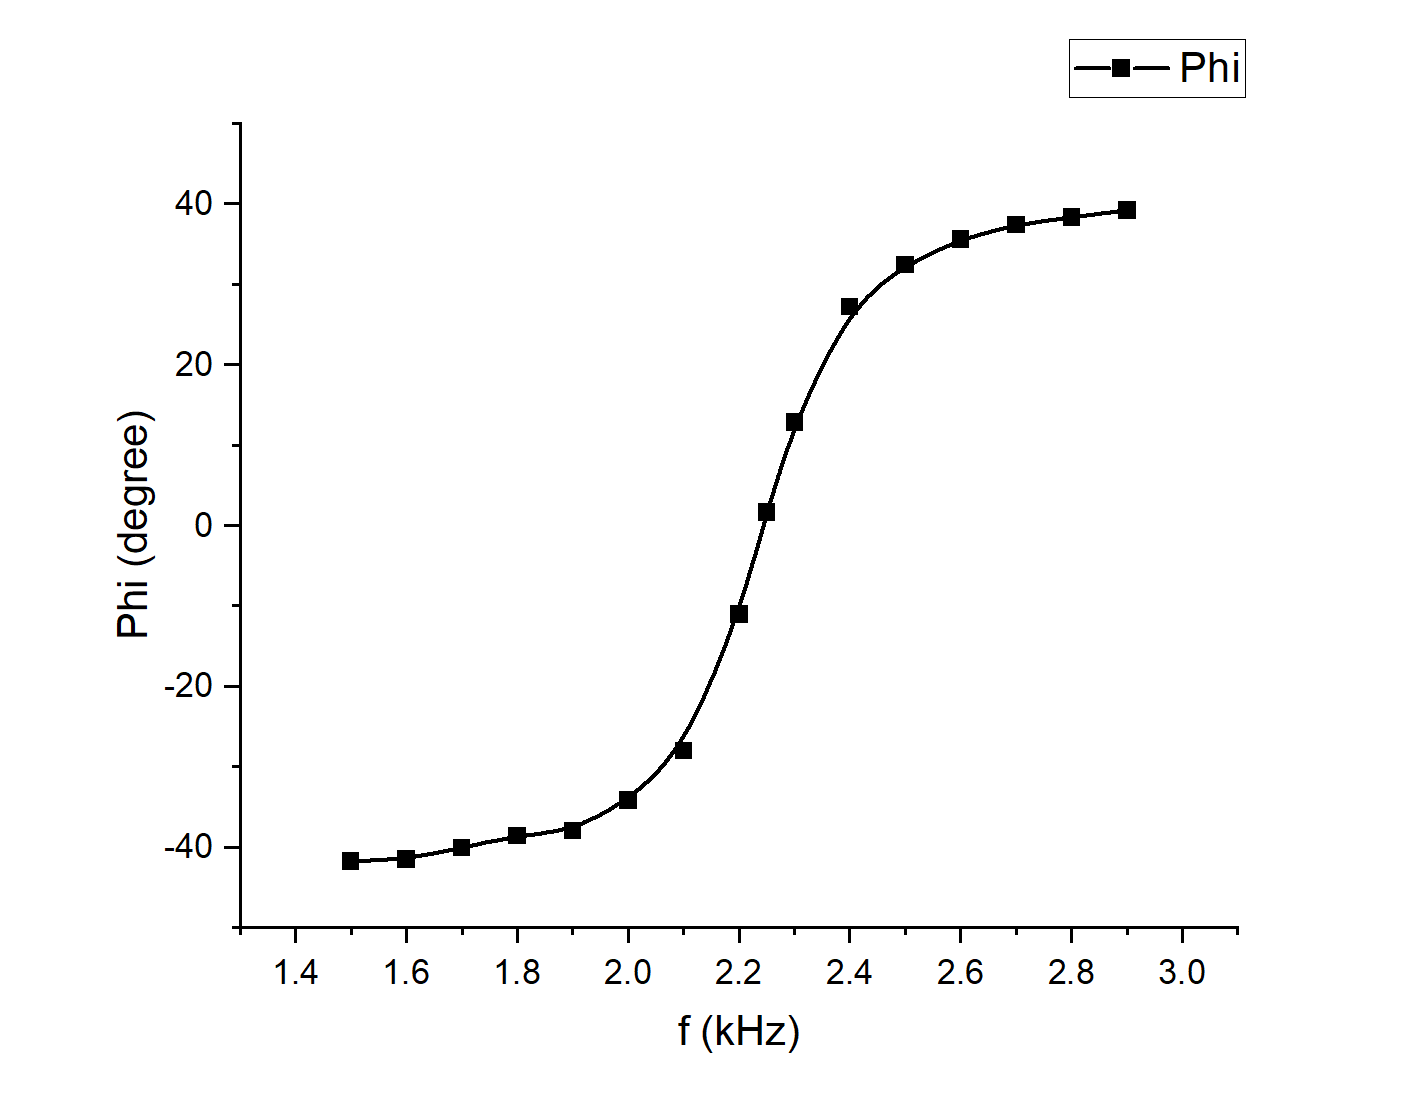
\includegraphics[width=8cm]{phi.png}
		\caption{相频特性曲线}
	\end{figure}
	当$\phi=0$时系统处于谐振状态,由图知
	\begin{align}
		f_{02}=2.244\mathrm{kHz}
	\end{align}
	\begin{figure}[H]
		\centering
		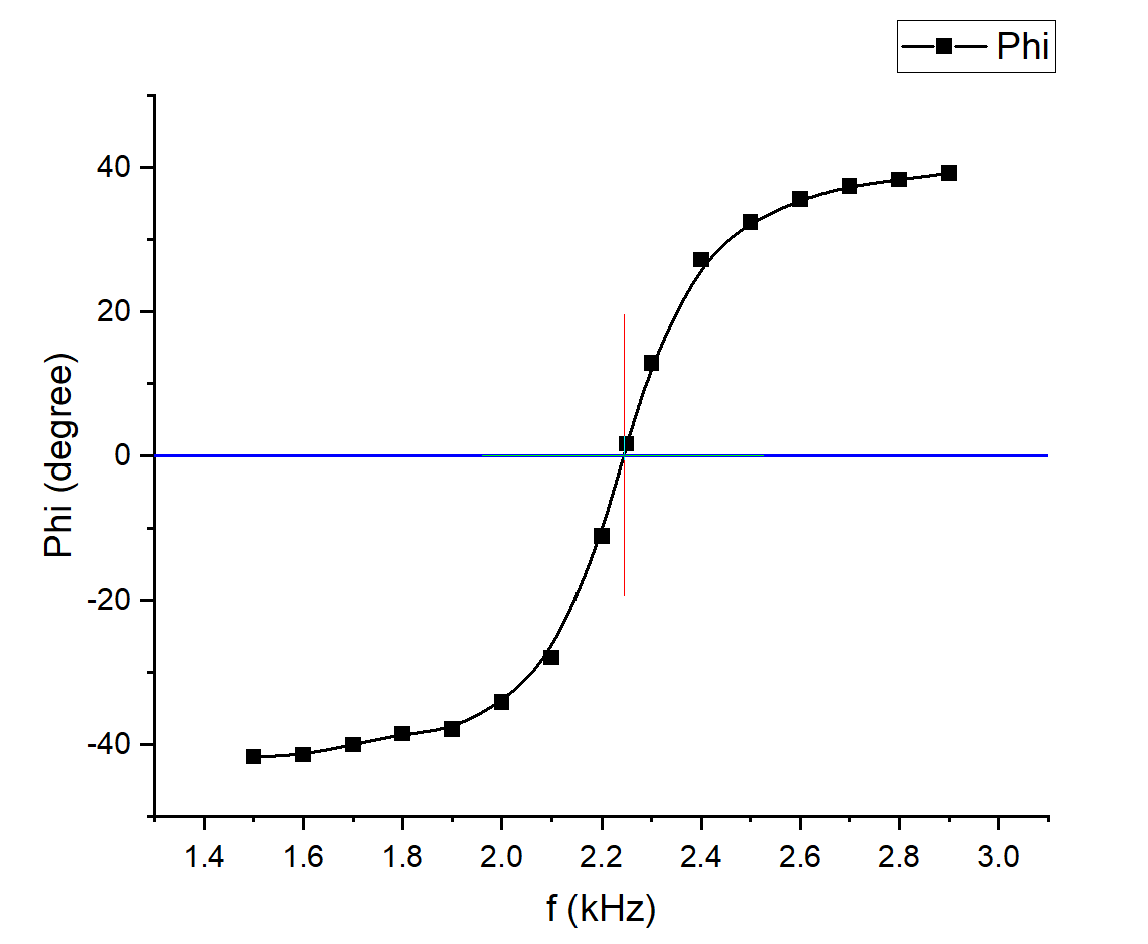
\includegraphics[width=8cm]{phi1.png}
		\caption{谐振频率的第二种测量}
	\end{figure}
	\subsection{幅频特性的测量以及谐振频率、品质因数的第三种计算方式}
	改变频率,用万用表测量电阻电压以及信号发生器两端电压并作比,用该比值$\alpha$代替电流作为幅频特性的体现
	\begin{align}
		\alpha=\frac{u_R}{u_{in}}
	\end{align}
	可作出幅频特性曲线\footnote{同样,原始数据附在末尾}
	\begin{figure}[H]
		\centering
		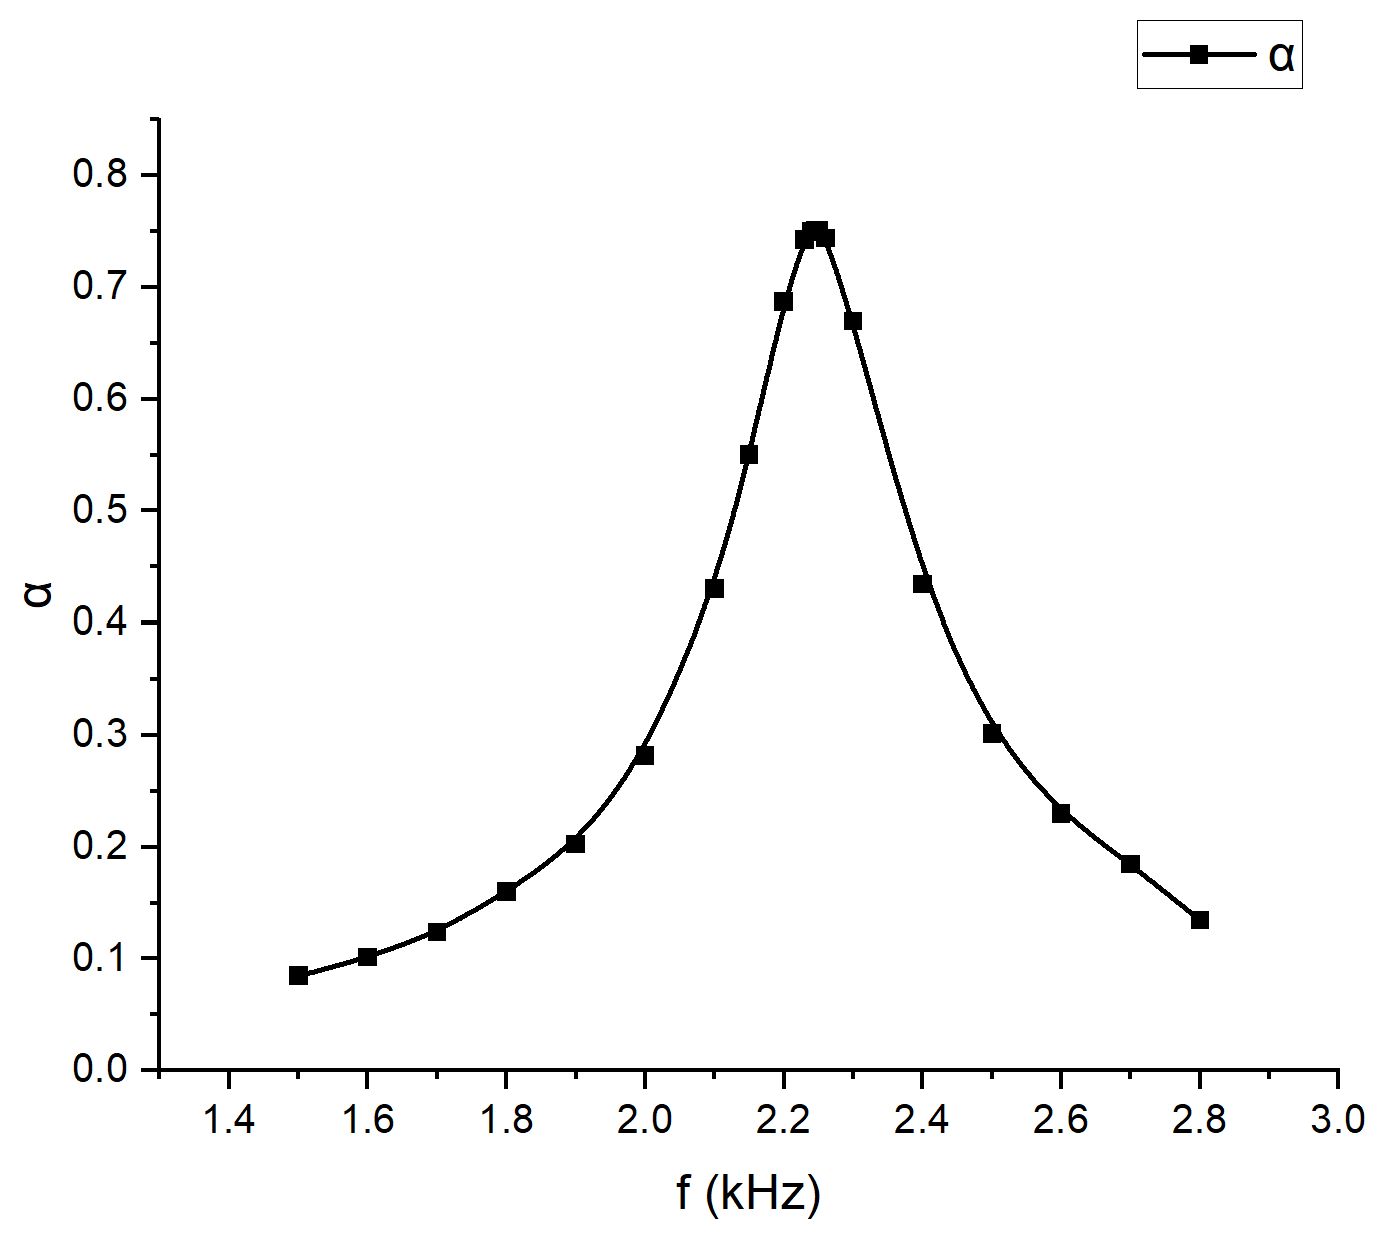
\includegraphics[width=8cm]{alpha.png}
		\caption{幅频特性曲线}
	\end{figure}
	同样地,可测量得到
	\begin{align}
		f_{03}=2.245\mathrm{kHz}
	\end{align}
	同时还可测量得到带宽
	\begin{align}
		\Delta f=f_2-f_1=2.360-2.141\mathrm{kHz}=0.219\mathrm{kHz}
	\end{align}
	\begin{align}
		Q_3=\frac{f_{03}}{\Delta f}=10.25
	\end{align}
	\begin{figure}[H]
		\centering
		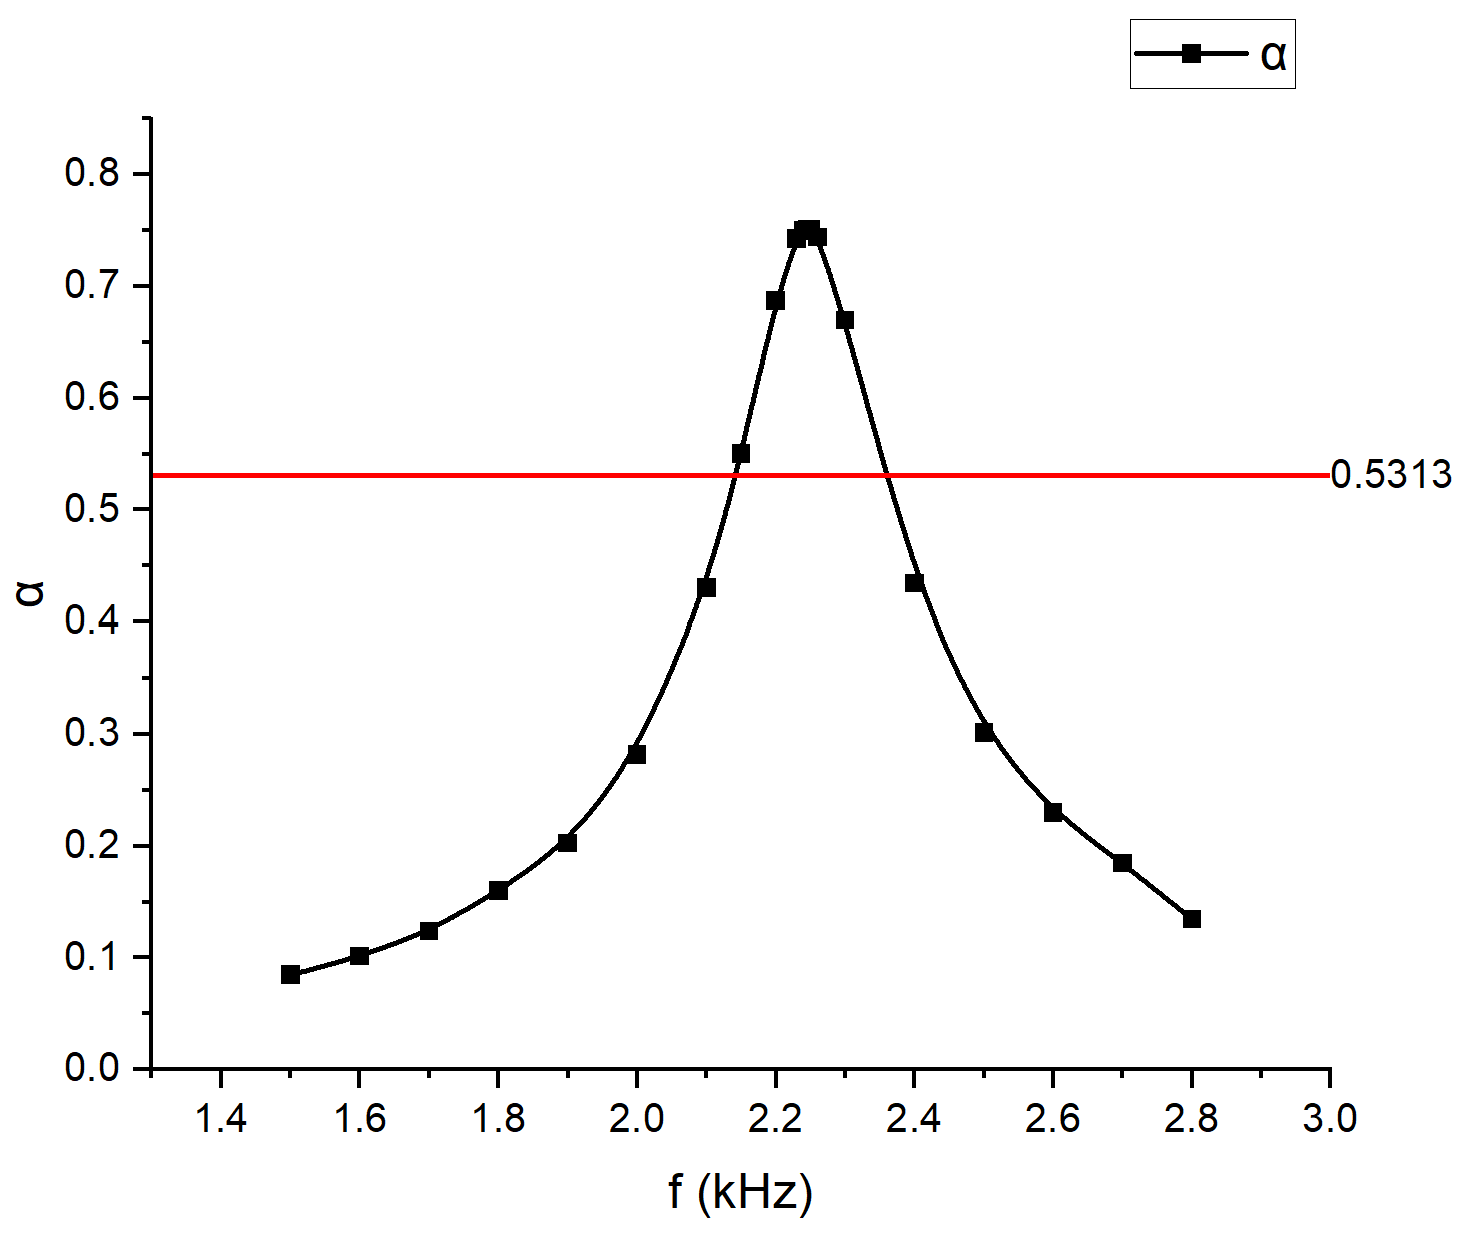
\includegraphics[width=8cm]{alpha1.png}
		\caption{谐振频率的第三种测量}
	\end{figure}
	\section{误差分析}
	\subsection{关于谐振频率的误差分析}
	通过电容和电感的值,我们可以计算出谐振频率的理论值
	\begin{align}
		f_{0,\mathrm{the}}=\frac{1}{2\pi\sqrt{LC}}=2.251\mathrm{kHz}
	\end{align}
	考虑电容和电感的不确定度
	\begin{align}
		\sigma_C&=C\times 0.65\%\\
		\sigma_L&=L\times 0.1\%
	\end{align}
	可得理论值的不确定度
	\begin{align}
		\sigma_{f_{0,\mathrm{the}}}=f_{0,\mathrm{the}}\sqrt{\left(\frac{\sigma_C}{2C}\right)^2+\left(\frac{\sigma_L}{2L}\right)^2}=0.008\mathrm{kHz}
	\end{align}
	可见我们所测量得到的三个谐振频率的值都在$(2.251\pm0.008)\mathrm{kHz}$区间内,结果是合理的。
	\subsection{关于品质因数的误差分析}
	关于品质因数,我们可以看到$Q_2$与$Q_3$的值相近,而与$Q_1$相差很多,这是因为我们在计算$Q_1$时只考虑了标准电阻和电感内阻,而没有考虑其他形式能量损耗所带来的“等效电阻”,实际上不是电阻,但是可以用电阻来等效。于是我们可以对$Q_1$的值进行一些修正。
	考虑谐振时,由测量的数据可以得到电阻电压与信号源电压之比
	\begin{align}
		\alpha_0=0.7513
	\end{align}
	实际上电路的电阻可以用下式计算
	\begin{align}
		R_{\mathrm{tot}}=R/\alpha_0=133.4\mathrm{\Omega}
	\end{align}
	然后再带进品质因数的第一种表达式里,可以得到
	\begin{align}
		Q'_{11}=10.58,Q'_{12}=10.62
	\end{align}
	从而我们可以得到相对统一的结果。
	\section{原始数据}
	\begin{figure}[H]
		\centering
		\includegraphics[width=14cm]{pic1.jpg}
	\end{figure}
	\begin{figure}[H]
		\centering
		\includegraphics[width=14cm]{pic2.jpg}
	\end{figure}
\end{document}